\documentclass[12pt]{article}

\usepackage[romanian]{babel}
\usepackage{hyperref}
\usepackage{graphicx}

\author{Tomas-Adrian Boboi, Alexandru-Vlad Cornea\\ Universitatea Politehnica Timișoara}
\date{2021}
\title{Proiect Sisteme Expert\\ \Large{Sistem expert pentru recomandarea unei configurații de sistem de calcul}}

\begin{document}
    
    \maketitle
    \thispagestyle{empty}
    \pagebreak

    \tableofcontents
    \pagenumbering{arabic}
    \pagebreak

    \section{Utilizarea aplicației}
    Ținta demografică a acestei aplicații este reprezentată de acei oameni care doresc să achiziționeze un sistem nou de calcul, având bine stabilit scopul pentru care va fi utilizat acest sistem, însă având un nivel de cunoștințe tehnice scăzut sau mediu. Având în minte aceste fapte, aplicația noastră oferă o recomandare de configurație de componente PC care să ruleze suita de aplicații specificată de utilizator.

    Pornirea aplicației se face rulând executabilul care a fost livrat împreună cu această documentație.

    La pornirea aplicației, utilizatorul trebuie să răspundă la două întrebări cu caracter general: trebuie să specifice un buget în care să se încadreze recomandarea, și mai trebuie să specifice și categoria generală de aplicații pe care intenționează să le folosească. Software-ul nostru oferă trei categorii posibile: \textit{gaming}, pentru pasionații de jocuri, \textit{design}, pentru cei ce activează în domeniul editării grafice, respectiv \textit{office}, pentru cei care vor folosi sistemul de calcul pentru munca de birou.

    După răspunderea la aceste întrebări generale, utilizatorul este condus la întrebări specifice, care depind de categoria aleasă la punctul anterior.

    În cazul în care utilizatorul dorește un calculator de gaming, acesta este întrebat ce fel de jocuri dorește să ruleze, și la ce fel de performanțe se așteaptă.

    În cazul în care  utilizatorul dorește un calculator de design, acesta este întrebat ce fel de aplicații de editare (foto, video, 3D, etc.) dorește să ruleze.

    În cazul în care  utilizatorul dorește un calculator pentru munca de birou, întrucât aplicațiile care rulează în general pe astfel de sisteme nu au cerințe foarte mari, utilizatorul este întrebat doar dacă dorește ca spațiul de stocare să fie optimizat pentru dimensiune (de exemplu dacă se dorește stocarea unui număr foarte mare de documente sau fișiere multimedia), viteză (de exemplu dacă de dorește stocarea unui număr mai mic de fișiere, însă care sunt copiate și mutate frecvent), sau ambele (pentru o experiență fără compromisuri).
    \pagebreak

    \section{Documentație tehnică}
    În cadrul acestui proiect, am decis să urmăm structura clasică a unui sistem expert, care este împărțit în trei mari părți: \textit{interfața cu utilizatorul}, \textit{mașina de inferență} și \textit{baza de cunoștințe}.

    Scopul interfeței cu utilizatorul este de a pune întrebări acestuia, și de a primi răspunsurile, care vor fi procesate și trimise mai departe la mașina de inferență. Mașina de inferență ia aceste răspunsuri și aplică reguli logice pe datele existente în baza de cunoștințe, obținând astfel concluzii noi. Baza de cunoștințe este formată din date culese de la expertul uman în domeniu.

    În continuare vom trata fiecare componentă individual, urmărind detaliile fiecăreia de implementare, și relevând locul lor în cod.

        \subsection{Interfața cu utilizatorul \textit{(User interface)}}
        Interfața cu utilizatorul este compusă din ferestre de tipul \textit{Windows Forms}, cu care utilizatorul interacționează în cadrul procesului de răspundere la întrebări. Aceste ferestre conțin elemente de tipul \textit{ListBox}, \textit{ComboBox} și \textit{NumericUpDown}, cu ajutorul cărora utilizatorul poate selecta și introduce răspunsuri la întrebări, răspunsuri care sunt trimise mai apoi înspre mașina de inferență.

        \subsection{Mașina de inferență \textit{(Inference machine)}}
        Mașina de inferență reprezintă componenta sistemului responsabilă cu citirea și interpretarea regulilor din baza de cunoștințe, luând în calcul răspunsurile date de utilizator.

        În cadrul acestui proiect, am ales implementarea unei mașini de inferență bazată pe principiul \textit{Backwards chaining}. Această implementare implică parcurgerea tuturor regulilor, verificarea concluziei, și încercarea de activare a regulii prin procesul de \textit{matching} dintre premisele regulii curente și premisele generate de răspunsurile utilizatorului.

        În cazul în care toate premisele sunt întrunite (acestea fiind legate între ele prin operația logică \textit{AND}), regula este activată, iar concluzia este considerată validă. În cazul în care cel puțin o premisă nu este îndeplinită, sau o premisă care vine din partea utilizatorului nu trebuie să fie îndeplinită, regula rămâne inactivă, concluzia sa fiind incompatibilă cu cerințele utilizatorului.

        \begin{figure}
            \centering
            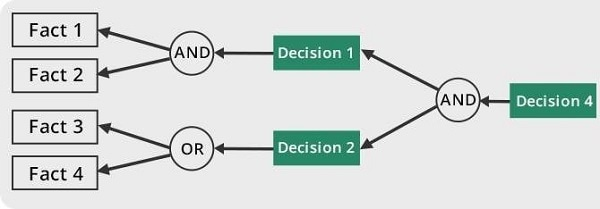
\includegraphics[width=\textwidth]{images/back_chain.png}
            \caption{Principiul de funcționare a unei mașini de inferență bazate pe backwards chaining. Pornind de la concluzii, mașina încearcă să găsească o potrivire între setul de premise de intrare și setul de premise al regulii, activând regula în cazul găsirii unei astfel de potriviri.}
        \end{figure}

        Bineînțeles, datorită numărului foarte mare de configurații de componente PC posibile, și datorită numărului și mai mare de combinații posibile de premise de intrare, combinate cu numărul mic de reguli, există posibilitatea (statistic foarte probabilă) ca sistemul să nu poată recomanda o configurație. Acest lucru se întâmplă în momentul în care mașina de inferență epuizează toate regulile, iar nicio concluzie nu a fost activată. În acest caz, utilizatorul trebuie să facă anumite compromisuri, pentru "a-i fi mai ușor" sistemului să vină cu o recomandare.

        \subsection{Baza de cunoștințe \textit{(Knowledge Base)}}
        Baza de cunoștințe reprezintă locul în care sunt stocate regulile, care provin de la expertul uman.

        În cadrul acestei implementări, baza de cunoștințe este stocată într-o bază de date locală, însă tehnologia folosită permite și stocarea cunoștințelor online, prin intermediul unui sistem de hosting. Acest lucru ar permite accesul la baza de date a oricărui utilizator cu o conexiune la internet, și ar permite creearea unei baze de cunoștințe mult mai vaste, întrucât dimensiunea acesteia nu mai este limitată de spațiul disponibil de stocare al utilizatorului final.

        Accesul la baza de cunoștințe se face prin intermediul directivelor SQL. Aducerea bazei de cunoștințe în memoria aplicației este urmată de procesul de \textit{parsing}, proces care transformă informațiile aduse de rutinele SQL într-un format inteligibil de către mașina de inferență. În urma procesului de \textit{parsing}, rezultă obiecte ale căror atribute sunt citite (și procesate) de mașina de inferență.

        Regulile din baza de cunoștințe au următoarea structură:
        \begin{itemize}
            \item{fiecare regulă are 32 de câmpuri corespunzătoare antecedentelor (premiselor), dintre care putem da câteva exemple:}
                \begin{itemize}
                    \item{RULE\_APPL\_GAMING - sistemul recomandat trebuie să fie un calculator de gaming}
                    \item{RULE\_GAMING\_RUN\_DECENT - jocurile selectate trebuie să ruleze decent (30-60 FPS) pe sistemul recomandat}
                    \item{RULE\_DESIGN\_ILLUSTRATOR - sistemul recomandat trebuie să fie capabil să ruleze aplicația Adobe Illustrator}
                    \item{RULE\_OFFICE\_AMBELE - sistemul recomandat trebuie să aibă spațiul de stocare optimizat atât pentru capacitate, cât și pentru viteză}
                \end{itemize}
            \item{fiecare regulă are un câmp corespunzător concluziei, câmp în care regăsim ID-ul PC-ului (fiecare configurație de componente are un ID unic) pe care îl va recomanda sistemul expert în cazul în care regula respectivă este activată}
        \end{itemize}

\end{document}